\chapter{Analysis}
\label{chapterreqass}
The chapter \textit{\nameref{chapterreqass}} consists of the three sections \textit{\nameref{gdpr}}, \textit{\nameref{sysrequirements}} and \textit{\nameref{cryptorequirements}}. \textit{\nameref{gdpr}} analyses the GDPR in order to identify regulations regarding this thesis and extract requirements. \textit{\nameref{sysrequirements}} models the process and workflows of the CliniScale project. The third section, \textit{\nameref{cryptorequirements}}, defines the used technical guidelines used for cryptographic protocols.

\section{General Data Protection Regulation}
\label{gdpr}
%data subject, data controller



This section analyses the statutory regulations implemented by the General Data Protection Regulation (GDPR).
The GDPR is a regulation on EU-law concerning data protection and privacy for all citizens of the European Union and the European Economic Area. Its goal is to give individuals more control over their personal data and simplifying the regulatory environment for private companies by unifying the legislation within the EU.
\\

Regulatory specifications concerning a system collecting and processing sensitive personal data in the scope of this thesis are identified.
This implies that regulations by the GDPR concerning other subjects, such as Designation of the data protection officer\cite{GDPR37} or Fines/Penalties\cite{GDPR84}, are not taken into account.
\\
\paragraph{Personal Data} Article 4 (1) defines personal data as any information relating to an identified or identifiable natural person. An identifiable natural person is defined as an entity that can be identified by the data directly or indirectly. Directly could be data such as name, identification number or similar. Data that can lead indirectly to identification are, among others, location data, online identifiers or factors specific to the physical, physiological, genetic, mental, economic, cultural or social identity of that person.\cite{GDPR4}

\paragraph{Sensitive Personal Data} Article 9 defines sensitive personal data as special categories of personal data. The term sensitive personal data is found in the recital 51. It is defined as personal data that is by nature sensitive in relation to fundamental rights and freedoms of a natural person. Sensitiveness of the data merits specific protection as their processing can lead to significant risks to fundamental rights. In paragraph 1 sensitive personal data is defined as data revealing racial or ethnic origin, political opinions, religious or philosophical beliefs, trade union membership, genetic data, biometric data, data concerning health or data concerning a natural person's sex life or sexual orientation. The processing is prohibited per default and is only possible if specific rules defined in paragraph 2 apply. The only rule of interest for this thesis of the paragraph 2 for the processing of health data in the context of the CliniScale is defined in (a). Paragraph 2 (a) allows processing if the data subject has given explicit consent and no Union or Member State law prohibits lifting the prohibition of paragraph 1.\cite{GDPR9}\cite{GDPRrec51}

\paragraph{Lawfulness of Processing} Defined in article 6 of the GDPR. The article defines under which conditions the processing of personal, and sensitive, data is lawful. Paragraph 1 defines six conditions that may apply to a company: the data subject has given consent to the processing, processing is necessary for the performance of a contract the data subject is part of, processing is necessary for compliance with a legal obligation of the controller, processing is needed in order to protect vital interests of the data subject, processing is necessary to carry out a task carried out in public interest or by official authority in the controller and if processing is necessary for the purpose of the legitimate interests of a controller or third party. Only the first condition, consent by the data subject, is applicable to the CliniScale project.\cite{GDPR6}

\paragraph{Conditions for Consent} Article 7 and recital 32 define the conditions for consent. Consent must be given by a clear affirmative act by the data subject that is free given, specific, informed and unambiguous. It can be given in the form of a written statement, including by electronic means, or an oral statement. In order to obtain freely given consent, the data subject must have a real choice. Any element of inappropriate pressure or influence renders the consent invalid. For a consent to be specific and informed, the data subject must be informed on the controller’s identity, what kind of data will be processed for what use and for which purpose. Additionally, the data subject must be informed about his right to withdraw consent at any time. The consent must be bound to one or several clearly defined purposes, which have been sufficiently explained to the data subject. Last, the consent has to be unambiguous. It requires either a statement or a clear affirmative act.\cite{GDPR7}\cite{GDPRrec32}

\paragraph{Security of Processing} The term defined in article 32 places the responsibility on the controller to implement appropriate technical and organizational measures to secure personal data. \\
Paragraph 1 details four measures to ensure data privacy and security. Paragraph 1 (a) advocates to pseudonymization and encryption of personal data. Paragraph 1 (b) recommends measures to ensure the ongoing confidentiality, integrity, availability and resilience of processing systems and service. Paragraph 1 (c) includes measures to restore availability and access in a timely manner in case of a physical or technical incident. Last, paragraph 1 (d) recommends regularly testing, assessing and evaluation of the effectiveness of measures that ensure data privacy and security. These recommendations shall be implemented by the controller based on the risks to rights and freedoms of the data subjects. It is to note, that the GDPR gives no recommendation on which standards, protocols or configurations to use. The only requirement is to choose measurements by evaluating the state of the art, cost of implementation and the nature, scope, context and purpose of the processing. To determine what exactly falls under state of the art, it is recommended to rely on security standards or IT-security guidelines. \\
Paragraph 2 defines that the choice of security measures should be made by assessing an appropriate level of security based on the risks present to specific processing of personal data based on accidental or unlawful destruction, loss, alteration, unauthorized disclosure or access to personal data transmitted, stored or otherwise processed. This means that a controller has to implement appropriate measures depending on the risks present to a process or personal data. \\
Paragraph 3 recommends complying with the code of conduct, defined in article 40\cite{GDPR40}, or make use of certification, described in article 42 \cite{GDPR42}, to demonstrate compliance with the requirements set in paragraph 1.\\
Paragraph 4 binds the controller to implement a process or measurements to ensure that any person acting under the authority of the controller or the processor who has access to personal data does not process them except on instruction of the controller.\\
Using encryption as a measurement has additional benefits for the controller. In case of a data breach, authorities positively consider the use of encryption in their decision of whether and of what amount a fine is imposed.\cite{GDPR32}

\paragraph{Data Protection by Design and by Default} These principles are defined in article 25 of the GDPR. It defines the responsibility of the controller to implement the data protection principles  privacy by design and privacy by default. These measurements could consist of data minimization, pseudonymization of personal data as soon as possible, transparency of functions and processing of personal data or enabling the data subject to monitor the processing of his data.\cite{GDPR25}

In summary, requirements to the CliniScale project to comply with the GDPR can be defined.

\begin{itemize}
    \item[1] Personal and sensitive personal data has to be secured in a manner appropriate for the risks resulting in a loss of confidentiality, integrity or availability of the data.
    \item[2] State of the art measurements have to be implemented, such as cryptography or pseudonymization.
    \item[3] In order to gather and process personal data, consent of the user is required in a way of a clear affirmative act by the data subject that is freely given, specific, informed and unambiguous.
    \item[4] Data protection should be by design and by default.
\end{itemize}

A security risk assessment following the MoRA methodology implements security measurements based on the damage potential of an element for every security goal identified. This implies that data is secured in an appropriate way depending on the risks they provoke.\\
Implemented measurements follow technical guidelines recommending state of the art protocols. For further information see \textit{\nameref{cryptorequirements}}.\\
The act of obtaining consent of a user is out of the scope of this thesis. Therefore, it is assumed consent is given in a way complying the requirements of the GDPR.\\
By performing a security risk assessment in the early stages of development, the practice of security by design is applied from the beginning. Security by default is a property that the CliniScale team has to ensure in process of implementation.



\section{CliniScale System Process}
\label{sysrequirements}

In this section the process and workflow of the CliniScale project is defined.
\\
The infrastructure of the CliniScale Project is designed as a classic Client-Server model. This means it is a distributed application infrastructure with the server as a provider of services and resources and the client as service requester. In this case, two kind of clients request different services and resources from the CliniScale back end. The participating parties and their interaction are listed below:

\paragraph{CliniScale Environment} The server application consists of two services: the back end service and the TrialConfigurator. 
The TrialConfigurator offers the Trial Executor the service to create and configure a trial and select possible probands to perform the trial. Information about the probands is send to the Trial Executor in the form of ProbandData. ProbandData contains a list of possible probands the Trial Executor can choose from to perform the trial on. 
The Trial Executor creates a trial fitting his needs and sends the TrialConfiguration back to the TrialConfigurator. 
The back end service offers probands the service to register for the configured trial by using the CliniScale Application for mobile phones. After registration, the back end service sends the TrialConfiguration to the mobile application. As the proband performs the trial, information containing answers to surveys and the health data from measurements is gathered. These data are bundled as HealthData and send back to the back end service. 
After the configured trial period is over, the back end service bundles collected data of the probands and creates a report for the Trial Executor. This TrialResults is send to the Trial Executor.

\paragraph{Trial Executor} The Trial Executor is able to create and configure a clinical trial by using the TrialConfigurator. In the process of creating a trial, ProbandData is send from the Trial Configurator to the Trial Executor. ProbandData contains information about possible probands the Trial Executor can choose from to perform the clinical trial. When the Trial Executor finished configuring the trial, TrialConfiguration is send to the Trial Configurator.

\paragraph{CliniScale Application} The application for mobile phones enables probands to register for trials and collect trial results. Is a proband chosen to participate in a trial, the CliniScale back end service sends the TrialConfiguration to the CliniScale Application. The proband performs the clinical trial and collects data in the process. This data is sent back to the CliniScale back end service.

Following the defined process, the following things can be defined to model the system architecture. The system consists of three parties, the CliniScale Environment, the Trial Executor and the CliniScale Application representing the probands. The CliniScale environment consists of two services, the TrialConfigurator and the CliniScale back end. The TrialConfigurator has a connection to the Trial Executor, to enable the creation of a clinical trial. The CliniScale back end service has connections to both the Trial executor, to deliver the results to the trial, and the CliniScale Application, in order to perform the clinical trial. The Figure \ref{fig:cliniscalesystem} represents a basic model of the defined process.

\begin{figure}[H]
  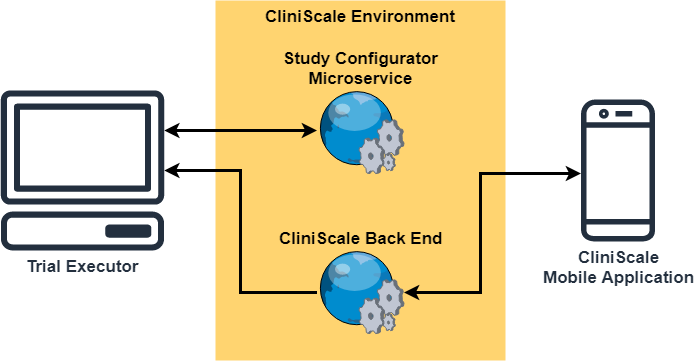
\includegraphics[width=\linewidth]{images/cs-flowchart.png}
  \caption{CliniScale Process Architecture}
  \label{fig:cliniscalesystem}
\end{figure}


\section{Technical Guidelines for Cryptographic Protocols}
\label{cryptorequirements}

The section \textit{\nameref{cryptorequirements}} identifies a technical guideline used as source of information when choosing cryptographic protocols and standards. The GDPR specifies the use of state of the art cryptographic protocols, without specifying which protocols or standards exactly to use and how to configure them. The GDPR recommends using proven standards and IT-security guidelines.
\\
The German Federal Office for Information Security (BSI) published technical guidelines\cite{bsitr} for cryptographic mechanisms assessing the security of different cryptographic protocols. From the various published guidelines, BSI TR-02102-1\cite{bsitr01} and BSI TR-02102-2\cite{bsitr02} are the ones relevant for this thesis. 
\\
BSI TR-02102-1 presents general recommendations for the choice of basic protocols and the right configuration of them, especially regarding the critical key length. 
\\
BSI TR-02102-2 concerns itself with the Transport Layer Security (TLS), a protocol which is commonly used for the transportation of data in the internet.
\\
The goal of the BSI technical guidelines is to spread appropriate security standards. Being updated regularly they provide a reliable source for information about state-of-the-art cryptographic protocols and their configuration that can be used in this thesis.
\\
